% vim: set filetype=tex:
%% Guidebook latex header
% Changelog
%   29.08.2015:
%           - Added footmisc pkg wegen footnote options in Tabellen bei der Packliste für den Transalp
%   30.08.2015:
%           - Added csquotes pkg für komische Keyboardlayouts ohne quotes
\documentclass[
	  DIV=12
	, a4paper
	, fontsize=10pt
	, footinclude
	, headinclude
	, plainfootsepline
]{scrartcl}

% german spelling
\usepackage[ngerman]{babel}

% fontenc VOR inputenc
\usepackage[T1]{fontenc}

% utf8 document
\usepackage[utf8]{inputenc}

% custom headers/footers
\usepackage{scrpage2}

% colors by names
\usepackage[usenames,dvipsnames,svgnames,table]{xcolor}

% title modification
\usepackage{titlesec}

% line spacing
\usepackage{setspace}

\usepackage{csquotes}

% nice Palatino font with old styled numbers
\usepackage[osf]{mathpazo}
% Palatino needs more leading (space between lines)
\linespread{1.15}

% use fullpage and exact margins
\usepackage[
%showframe
, top=1.9cm, bottom=2.5cm
, left=1.9cm, right=1.9cm
, footskip=0.9cm
, headheight=0cm
]{geometry} % passt soweit 01.2016
% old
%\usepackage[showframe, top=1.9cm, bottom=3.3cm, left=1.9cm, right=1.9cm, headheight=0cm]{geometry} % passt soweit 05.2014


% spaltige TOC
\usepackage[toc]{multitoc}

% text wrapping for pictures
\usepackage{wrapfig}
\usepackage{subcaption}
\captionsetup[wrapfigure]{labelformat=empty}
\captionsetup[subfigure]{labelformat=empty}

\usepackage[]{graphicx}
%\usepackage[draft]{graphicx}


\usepackage{overpic}
\usepackage{epstopdf}
%\usepackage[update,prepend]{epstopdf}

\usepackage{footmisc}


\usepackage{tabularx}
\usepackage{multirow}
\usepackage{nicefrac}
\usepackage[export]{adjustbox}
\usepackage[space]{grffile} % spaces in dateinamen
%\setkeys{Gin}{resolution=300} %set resolution of pics to 300dpi...?!
%\setkeys{Gin}{resolution=72}
\pdfimageresolution=300
% newline in table cells
\usepackage{pbox}
% Transparent Hoehenprofil
\usepackage{transparent}
\usepackage{eso-pic}
\usepackage{picture}

%\usepackage{pgfpages}
\usepackage{pdfpages}


% math packages
\usepackage{amsmath,marvosym,textcomp,wasysym,amssymb}
%\usepackage{amsmath,marvosym,textcomp}

% arabische zaehlweise der subsection
\renewcommand{\thesubsection}{\arabic{subsection}}

% MTB       Maroon    #AF3235
% Skitour   RoyalBlue #006EB8
\definecolor{skitour}{RGB}{0,110,184}
\definecolor{mtb}{RGB}{175,50,53}
\definecolor{einkehr}{RGB}{60,128,49}
\definecolor{wandern}{RGB}{0,155,85}

\titleformat*{\subsection}{\normalfont\huge\bfseries\color{Maroon}}
\titleformat*{\subsubsection}{\normalfont\large\bfseries\color{Maroon}}

% \nosection tauchen nicht im text auf
\newcommand{\nosection}[1]{%
  \refstepcounter{section}%
  \addcontentsline{toc}{section}{\protect\numberline{}#1}%
  \markright{#1}}
\makeatletter
\newcommand\invisiblesection[1]{%
  \refstepcounter{section}%
  \addcontentsline{toc}{section}{\protect\numberline{\thesection}#1}%
  \sectionmark{#1}\phantom{}}
\makeatother

\usepackage{layouts} % get the \textwidth in cm
% == 15.91774cm

\usepackage{lastpage}


\pagestyle{scrplain}
\clearscrheadfoot{}
\ifoot[\rightmark]{}
\setfootsepline{.6pt}


\usepackage{booktabs}
\usepackage{dcolumn}
\usepackage{units}
\usepackage{array}
% fancy table stuff
\makeatletter
\newcommand{\armultirow}[3]{%
  \multicolumn{#1}{#2}{%
    \begin{picture}(0,0)%
      \put(0,0){%
        \begin{tabular}[t]{@{}#2@{}}%
          #3%
        \end{tabular}%
      }%
    \end{picture}%
  }%
}%

\newcolumntype{f}{>{$}l<{$}}
\newcolumntype{n}{l}
\newcolumntype{N}{>{\scriptsize}l}
\newcolumntype{v}[1]{>{\raggedright\hspace{0pt}}p{#1}}
\newcolumntype{V}[1]{>{\scriptsize\raggedright\hspace{0pt}}p{#1}}
%
% array.sty, dcolumn.sty
\newcolumntype{B}[1]{>{\boldmath\DC@{.}{,}{#1}}l<{\DC@end}}
\newcolumntype{b}[1]{>{\DC@{.}{,}{#1}}r<{\DC@end}}
\newcolumntype{d}[1]{>{\DC@{.}{,}{#1}}l<{\DC@end}}
\newcolumntype{s}[1]{>{\DC@{.}{,}{#1}\mathsf\bgroup}l<{\egroup\DC@end}}
%
% array.sty, rotating.sty
\newcolumntype{R}[1]{%
  >{\begin{turn}{90}\begin{minipage}{#1}\scriptsize\raggedright\hspace{0pt}}l%
  <{\end{minipage}\end{turn}}%
}
%
% array.sty, tabularx.sty
\newcolumntype{x}{>{\scriptsize\raggedright\hspace{0pt}}X}
\makeatother



%\begin{document}
\titleformat*{\subsubsection}{\normalfont\large\bfseries\color{skitour}}
\titleformat*{\subsection}{\normalfont\huge\bfseries\color{skitour}}

\subsection{Kleiner Daumen KL \small{2197m}}

% create header
\ohead[Fr, 20.03.2015]{}
\graphicspath{{skitouren/kl.daumen-20.03.2015//}}
\def \mypath{skitouren/kl.daumen-20.03.2015/}
\cfoot[\vspace{-0.7em}  Allgäu - Vorderes Ostrachtal ]{}
\ifoot[{\vspace{-2.7em} 
\includegraphics[scale=0.2]{meta/parkplatz/hinterstein.p} }]{}
\ofoot[\vspace{-0.7em} Winter 2014/2015 $~\bullet$ S. \pagemark ]{}

% create elevation profile
\AddToShipoutPicture*{
    \AtTextUpperLeft{
        \put(14,-130){
            \parbox[b][\paperheight]{\textwidth}{
                \raggedleft
                \adjustbox{max height=5.0cm, max width=.65\textwidth,keepaspectratio}{
                    % GNUPLOT: LaTeX picture with Postscript
\begingroup
  \makeatletter
  \providecommand\color[2][]{%
    \GenericError{(gnuplot) \space\space\space\@spaces}{%
      Package color not loaded in conjunction with
      terminal option `colourtext'%
    }{See the gnuplot documentation for explanation.%
    }{Either use 'blacktext' in gnuplot or load the package
      color.sty in LaTeX.}%
    \renewcommand\color[2][]{}%
  }%
  \providecommand\includegraphics[2][]{%
    \GenericError{(gnuplot) \space\space\space\@spaces}{%
      Package graphicx or graphics not loaded%
    }{See the gnuplot documentation for explanation.%
    }{The gnuplot epslatex terminal needs graphicx.sty or graphics.sty.}%
    \renewcommand\includegraphics[2][]{}%
  }%
  \providecommand\rotatebox[2]{#2}%
  \@ifundefined{ifGPcolor}{%
    \newif\ifGPcolor
    \GPcolortrue
  }{}%
  \@ifundefined{ifGPblacktext}{%
    \newif\ifGPblacktext
    \GPblacktexttrue
  }{}%
  % define a \g@addto@macro without @ in the name:
  \let\gplgaddtomacro\g@addto@macro
  % define empty templates for all commands taking text:
  \gdef\gplbacktext{}%
  \gdef\gplfronttext{}%
  \makeatother
  \ifGPblacktext
    % no textcolor at all
    \def\colorrgb#1{}%
    \def\colorgray#1{}%
  \else
    % gray or color?
    \ifGPcolor
      \def\colorrgb#1{\color[rgb]{#1}}%
      \def\colorgray#1{\color[gray]{#1}}%
      \expandafter\def\csname LTw\endcsname{\color{white}}%
      \expandafter\def\csname LTb\endcsname{\color{black}}%
      \expandafter\def\csname LTa\endcsname{\color{black}}%
      \expandafter\def\csname LT0\endcsname{\color[rgb]{1,0,0}}%
      \expandafter\def\csname LT1\endcsname{\color[rgb]{0,1,0}}%
      \expandafter\def\csname LT2\endcsname{\color[rgb]{0,0,1}}%
      \expandafter\def\csname LT3\endcsname{\color[rgb]{1,0,1}}%
      \expandafter\def\csname LT4\endcsname{\color[rgb]{0,1,1}}%
      \expandafter\def\csname LT5\endcsname{\color[rgb]{1,1,0}}%
      \expandafter\def\csname LT6\endcsname{\color[rgb]{0,0,0}}%
      \expandafter\def\csname LT7\endcsname{\color[rgb]{1,0.3,0}}%
      \expandafter\def\csname LT8\endcsname{\color[rgb]{0.5,0.5,0.5}}%
    \else
      % gray
      \def\colorrgb#1{\color{black}}%
      \def\colorgray#1{\color[gray]{#1}}%
      \expandafter\def\csname LTw\endcsname{\color{white}}%
      \expandafter\def\csname LTb\endcsname{\color{black}}%
      \expandafter\def\csname LTa\endcsname{\color{black}}%
      \expandafter\def\csname LT0\endcsname{\color{black}}%
      \expandafter\def\csname LT1\endcsname{\color{black}}%
      \expandafter\def\csname LT2\endcsname{\color{black}}%
      \expandafter\def\csname LT3\endcsname{\color{black}}%
      \expandafter\def\csname LT4\endcsname{\color{black}}%
      \expandafter\def\csname LT5\endcsname{\color{black}}%
      \expandafter\def\csname LT6\endcsname{\color{black}}%
      \expandafter\def\csname LT7\endcsname{\color{black}}%
      \expandafter\def\csname LT8\endcsname{\color{black}}%
    \fi
  \fi
    \setlength{\unitlength}{0.0500bp}%
    \ifx\gptboxheight\undefined%
      \newlength{\gptboxheight}%
      \newlength{\gptboxwidth}%
      \newsavebox{\gptboxtext}%
    \fi%
    \setlength{\fboxrule}{0.5pt}%
    \setlength{\fboxsep}{1pt}%
\begin{picture}(9680.00,4800.00)%
    \gplgaddtomacro\gplbacktext{%
      \colorrgb{0.00,0.00,0.00}%
      \put(222,159){\makebox(0,0){\strut{}0\scriptsize km}}%
      \colorrgb{0.00,0.00,0.00}%
      \put(3346,159){\makebox(0,0){\strut{}5\scriptsize km}}%
      \colorrgb{0.00,0.00,0.00}%
      \put(6470,159){\makebox(0,0){\strut{}10\scriptsize km}}%
      \colorrgb{0.00,0.00,0.00}%
      \put(8700,620){\makebox(0,0)[l]{\strut{}1000\scriptsize m}}%
      \colorrgb{0.00,0.00,0.00}%
      \put(8700,1251){\makebox(0,0)[l]{\strut{}1200\scriptsize m}}%
      \colorrgb{0.00,0.00,0.00}%
      \put(8700,1883){\makebox(0,0)[l]{\strut{}1400\scriptsize m}}%
      \colorrgb{0.00,0.00,0.00}%
      \put(8700,2515){\makebox(0,0)[l]{\strut{}1600\scriptsize m}}%
      \colorrgb{0.00,0.00,0.00}%
      \put(8700,3146){\makebox(0,0)[l]{\strut{}1800\scriptsize m}}%
      \colorrgb{0.00,0.00,0.00}%
      \put(8700,3778){\makebox(0,0)[l]{\strut{}2000\scriptsize m}}%
      \colorrgb{0.00,0.00,0.00}%
      \put(8700,4410){\makebox(0,0)[l]{\strut{}2200\scriptsize m}}%
    }%
    \gplgaddtomacro\gplfronttext{%
      \csname LTb\endcsname%
      \put(4786,4699){\makebox(0,0)[l]{\strut{}\textcolor{skitour}{Kl. Daumen \tiny 2197m}}}%
    }%
    \gplgaddtomacro\gplbacktext{%
    }%
    \gplgaddtomacro\gplfronttext{%
    }%
    \gplbacktext
    \put(0,0){\includegraphics{hoehenprofil}}%
    \gplfronttext
  \end{picture}%
\endgroup

                }
            }
        }
    }
}

\def\arraystretch{1.3} % bessere Lesbarkeit im Kopfteil
\vspace{-0.75em}
{\small  \setstretch{1.3}
% left table
\begin{tabularx}{0.5\textwidth}{X X X X X}
    \multicolumn{4}{c}{         \(\bigstar~\bigstar~\bigstar~\)}        \\
    $\uparrow$                1.365{\scriptsize hm} &
    $\rightsquigarrow$        13.4{\scriptsize km} &
    LLB                         1               \\
    \rule{0pt}{3ex} $\vec{t}$ 2:44{\scriptsize h} &
    $\Delta t$                4:39{\scriptsize h} &
    \Cross \space               3:40{\scriptsize h} \\
    \clock\space                6.15         &
    \multicolumn{2}{l}{ \smiley\space \pbox{2.8cm}{
        \scriptsize{            Jojo }}
    } \\

    \multicolumn{2}{c}{         \(ZS-\)/2.1/Ex2 }   &
    % empty lines for difficulty
                                                    &
                                                    \\
    & \multicolumn{2}{c}{       \framebox{P} Hinterstein (2.50\euro{}) }

\vspace{0.5em}
\end{tabularx}
}\\

% create map
\begin{wrapfigure}[28]{R}{0.46\textwidth}
    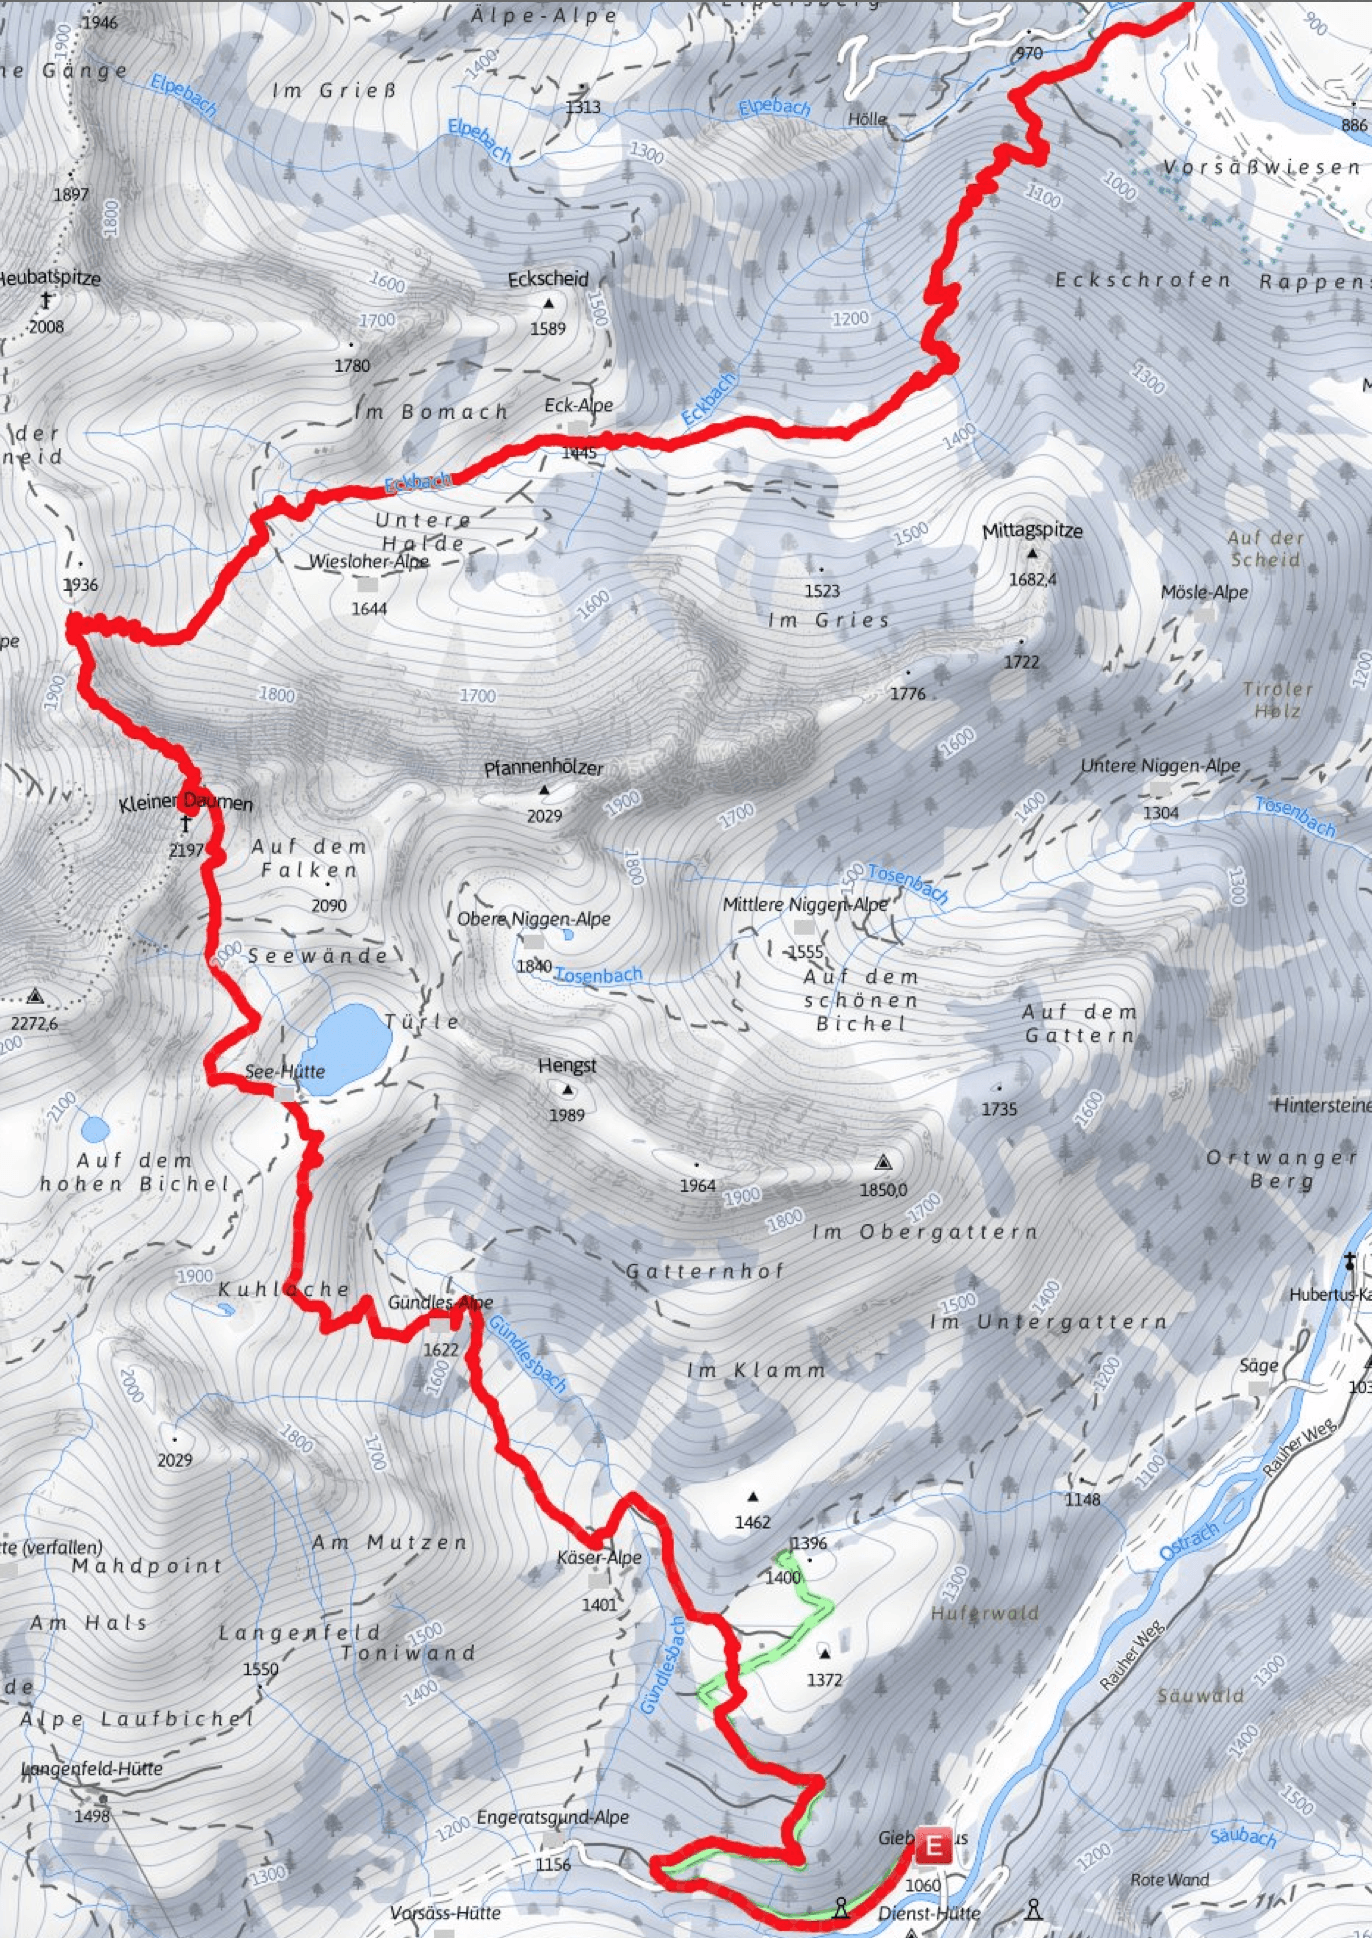
\includegraphics[frame, width=0.46\textwidth]{karteninfo}
    \vspace{-0.7em}
\end{wrapfigure}
\setstretch{1.0}

\blindtext[3]

\par 

\begin{wrapfigure}[13]{l}{0.43\textwidth}
\vspace{-1em}
    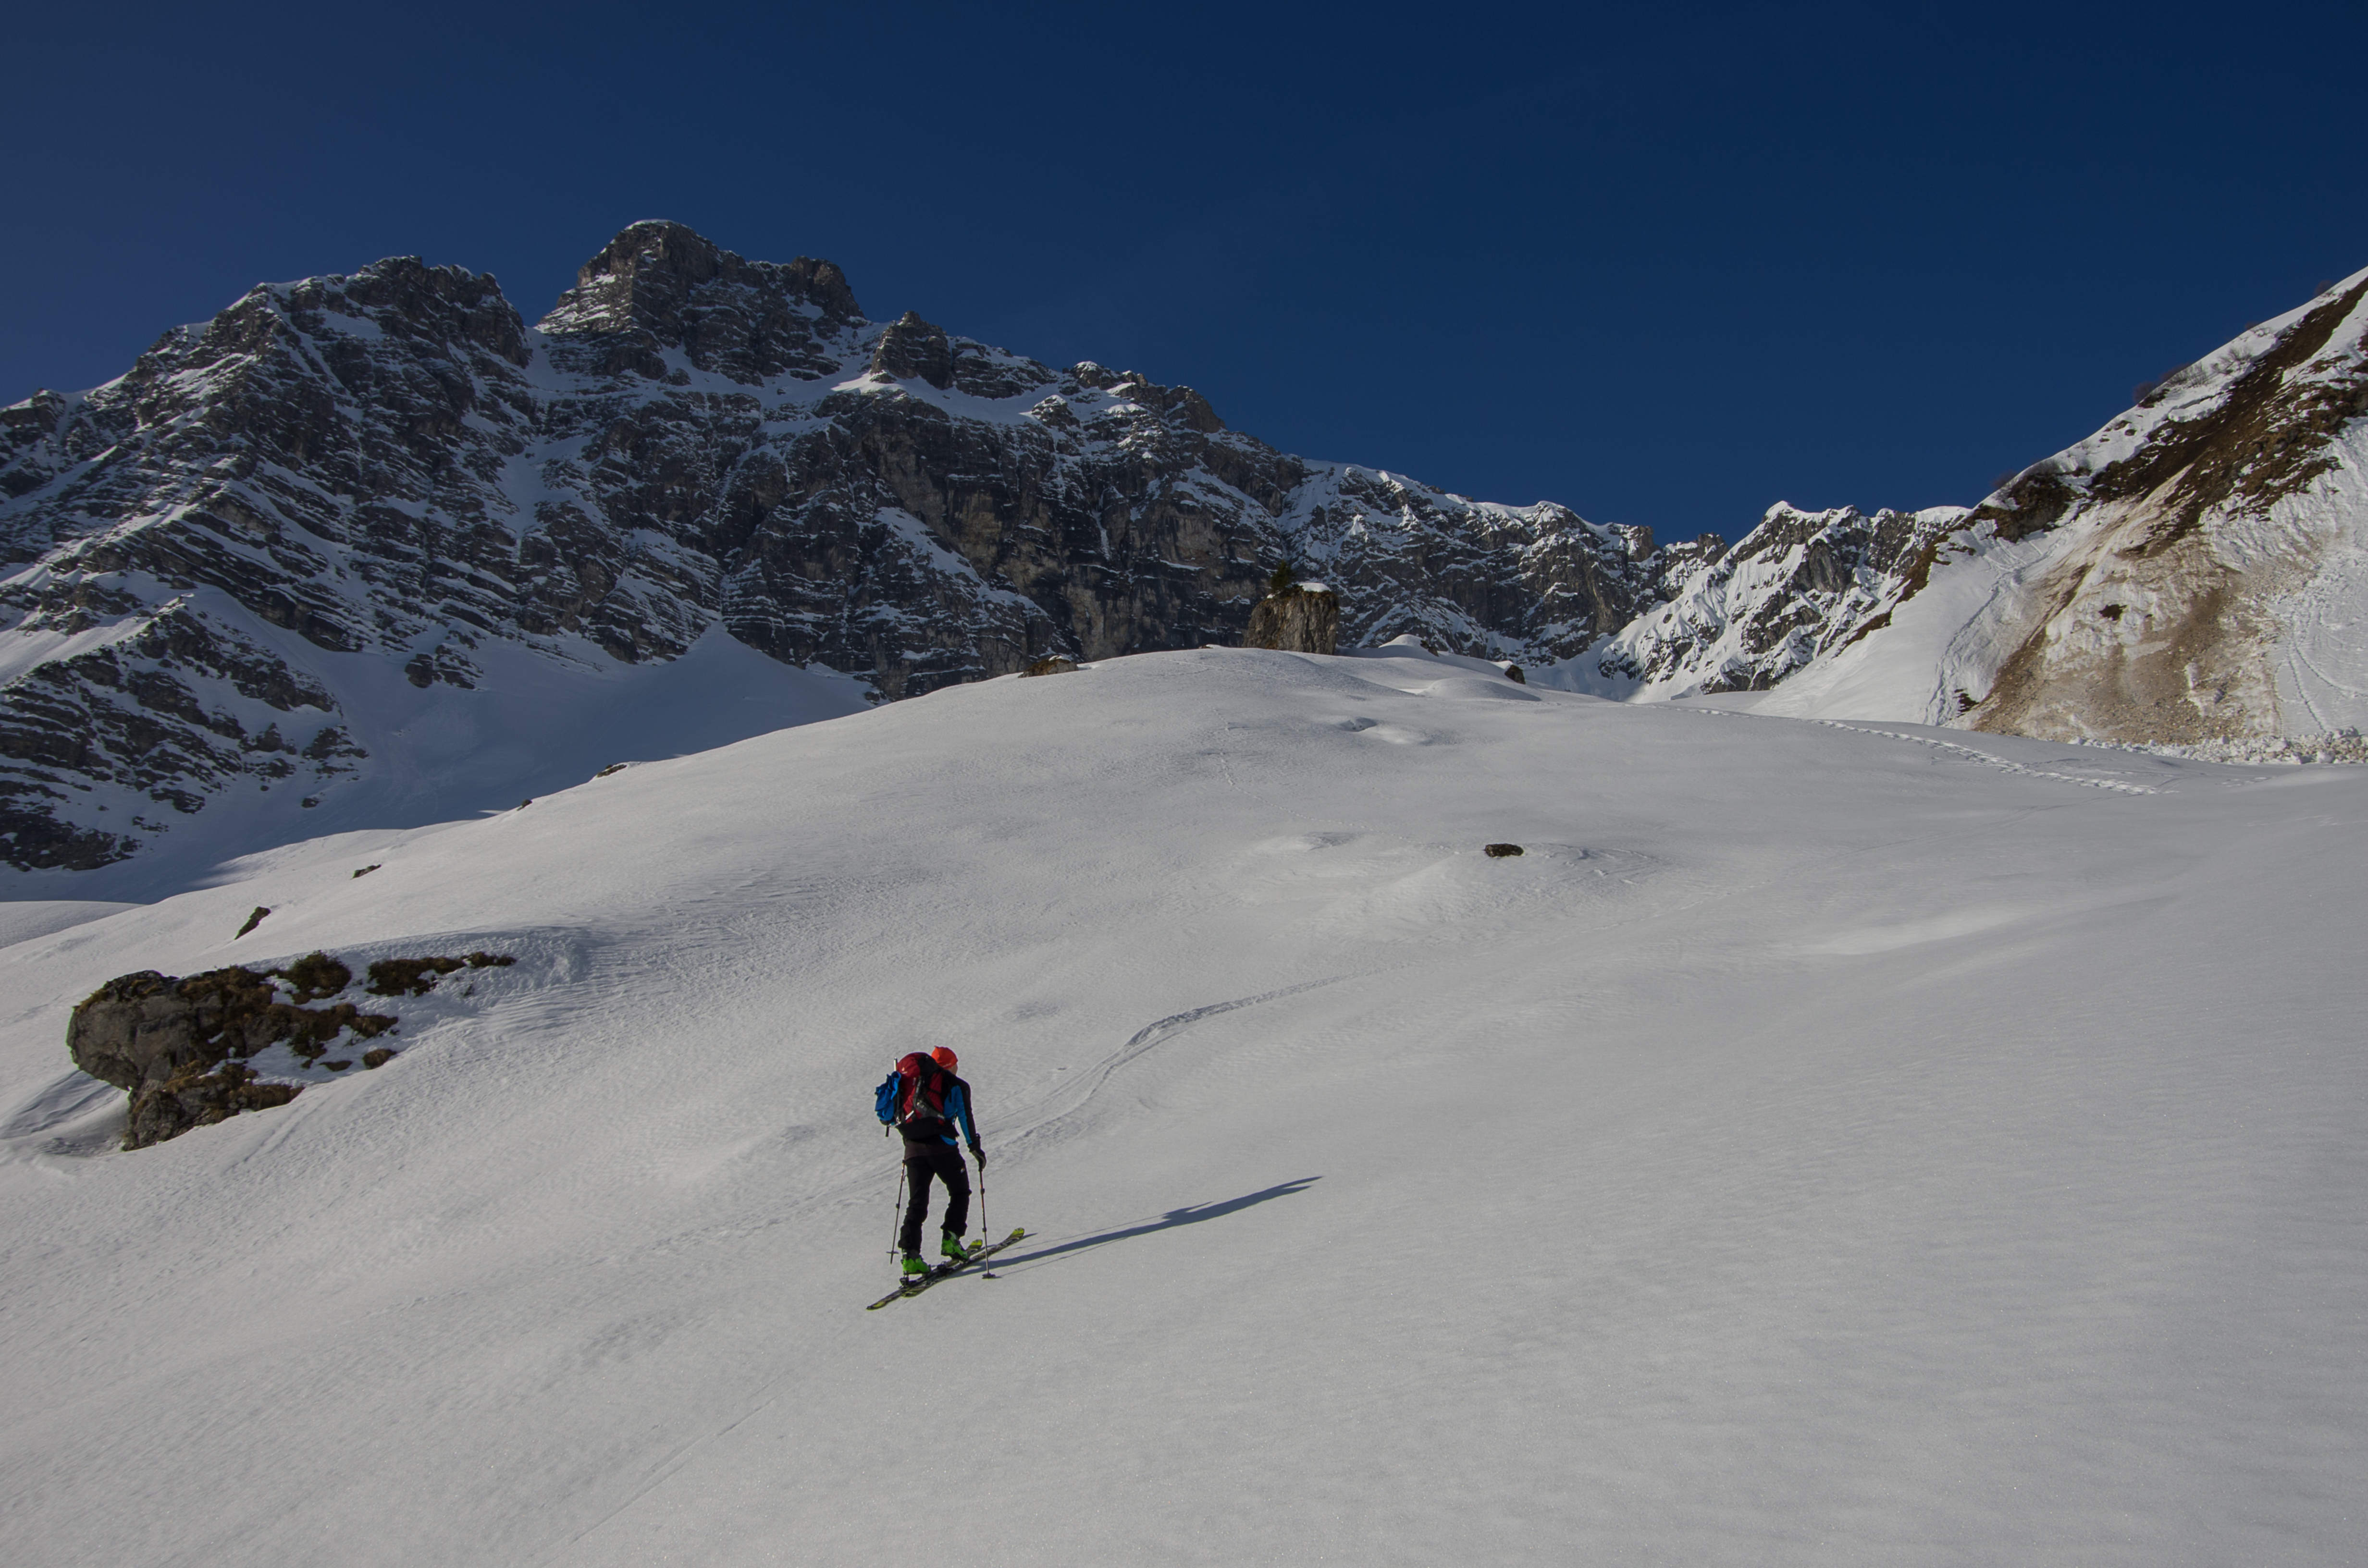
\includegraphics[width=0.42\textwidth]{\mypath/bilder/summit}
    \vspace{-3em}
\end{wrapfigure}

\noindent \(\blacktriangleright\) \blindtext

\clearpage

%\end{document}
